\documentclass[11pt]{article}
\usepackage{amsmath,amsbsy,amssymb,verbatim,fullpage,ifthen,graphicx,bm,amsfonts,amsthm,url}
\usepackage{graphicx}
\usepackage{xcolor}
\newcommand{\mfile}[1]  {{\small \verbatiminput{./#1}}} % Jeff Fessler, input matlab file
\newcommand{\tmop}[1]{\ensuremath{\operatorname{#1}}}
%\newcommand*{\qed}{\hfill\ensuremath{\blacksquare}}%
\newcommand{\R}{\mathbb{R}}
\newcommand{\C}{\mathbb{C}}
\newcommand{\Z}{\mathbb{Z}}
\newcommand{\A}{\mathcal{A}}
\newcommand{\minimize}{\operatorname*{minimize\ }}
\newcommand{\maximize}{\operatorname*{maximize}}
\newcommand{\opdet}[1]{\operatorname{\textbf{det}}\left(#1\right)}
\newcommand{\optr}[1]{\operatorname{\textbf{tr}}\left(#1\right)}
\newcommand{\mtx}[1]{\mathbf{#1}}
\newcommand{\vct}[1]{\mathbf{#1}}
\def \lg       {\langle}
\def \rg       {\rangle}
\def \mA {\mtx{A}}
\def \mF {\mtx{F}}
\def \mG {\mtx{G}}
\def \mI {\mtx{I}}
\def \mJ {\mtx{J}}
\def \mU {\mtx{U}}
\def \mS {\mtx{S}}
\def \mV {\mtx{V}}
\def \mW {\mtx{W}}
\def \mLambda {\mtx{\Lambda}}
\def \mSigma {\mtx{\Sigma}}
\def \mX {\mtx{X}}
\def \mY {\mtx{Y}}
\def \mZ {\mtx{Z}}
\def \zero     {\mathbf{0}}
\def \vzero    {\vct{0}}
\def \vone    {\vct{1}}
\def \va {\vct{a}}
\def \vg {\vct{g}}
\def \vu {\vct{u}}
\def \vv {\vct{v}}
\def \vw {\vct{w}}
\def \vx {\vct{x}}
\def \vy {\vct{y}}
\def \vz {\vct{z}}
\def \vphi {\vct{\phi}}
\def \vmu {\vct{\mu}}
\def \R {\mathbb{R}}

%\newcommand{\st}{\operatorname*{\ subject\ to\ }}
\usepackage{algorithm,algpseudocode}
\usepackage{xspace}
% Add a period to the end of an abbreviation unless there's one
% already, then \xspace.
\makeatletter
\DeclareRobustCommand\onedot{\futurelet\@let@token\@onedot}
\def\@onedot{\ifx\@let@token.\else.\null\fi\xspace}

\def\eg{\emph{e.g}\onedot} \def\Eg{\emph{E.g}\onedot}
\def\ie{\emph{i.e}\onedot} \def\Ie{\emph{I.e}\onedot}
\def\cf{\emph{c.f}\onedot} \def\Cf{\emph{C.f}\onedot}
\def\etc{\emph{etc}\onedot} \def\vs{\emph{vs}\onedot}
\def\wrt{w.r.t\onedot} \def\dof{d.o.f\onedot}
\def\etal{\emph{et al}\onedot} \def\st{\emph{s.t}\onedot}
\pagestyle{plain}

\title{{\bf Homework Set 5, CPSC 8420, Fall 2023}} % Change to the appropriate homework number
\author{\Large\underline{Last Name, First Name}}
\date{\textbf{\Large\textcolor{red}{Due 12/10/2023, Friday, 11:59PM EST}}} % put your name in the LastName, FirstName format
%\date{\today}

\begin{document}
\maketitle
\section*{Problem 1}
Recall the classification models we discussed in class: \textbf{SVM} and \textbf{Logistic Regression}, seems both of them work on binary classification task. However, in real-world applications, multi-classification is everywhere, thus in this problem we explore how to extend vanilla \textbf{Logistic Regression} for multi-classification. Assume we have $K$ different classes and the input $
\vx\in\mathcal{R}^d$, and the probability to each class is defined as:
\begin{equation}
	%\begin{aligned}
		P(Y=k|X=\vx) =  \frac{exp(\vw_k^T\vx)}{ 1+\sum_{l=1}^{K-1}exp(\vw_l^T\vx)} \quad for  \quad k=1,2,\dots,K-1; P(Y=K|X=\vx) =  \frac{1} { 1+\sum_{l=1}^{K-1}exp(\vw_l^T\vx)}
	%\end{aligned}
\end{equation}
If we define $\vw_K=\vzero$, then we can combine the two cases above as one:
\begin{equation}
	P(Y=k|X=\vx) =  \frac{exp(\vw_k^T\vx)}{ 1+\sum_{l=1}^{K-1}exp(\vw_l^T\vx)} \quad for  \quad k=1,\dots,K
\end{equation}
\begin{enumerate}
	\item What and how many parameters are there to be optimized? 
		$$ \{\vw_1,\vw_2 ... \vw_{k-1}\}$$ since each $\vw_i$ is a $d$ dimension vector,
		so total $d\times(k-1)$
	\item The training data is given as: $\{(\vx_1,y_1),\dots,(\vx_n,y_n)\}$, please simplify the log likelihood function to your best:

	\begin{align}
		L(\vw_1,\dots,\vw_{K-1})&=\sum\limits_{i=1}^n ln P(Y=y_i|X=\vx_i)\\
		&=\sum\limits_{i=1}^n ln \frac{exp(\vw_{y_i}^T\vx_i)}{1+\sum\limits_{l=1}^{K-1}exp(\vw_{l}^T\vx_i)}\\
		& = \sum\limits_{i=1}^n (\vw_{y_i}^T\vx_i - ln (1+\sum\limits_{l=1}^{K-1}exp(\vw_{l}^T\vx_i)))
	\end{align}


	\item Now please find the gradient of $L$ \wrt $\vw_k$.
	
	\begin{align}
		\frac{\partial L}{\partial \vw_k} = \sum\limits_{i=1}^n ( \mI(y_i==k)\vx_i -\frac{exp(\vw_k^T\vx_i)}{1+\sum\limits_{l=1}^{K-1}exp(\vw_{l}^T\vx_i)}\vx_i), y_i=k
	\end{align}


	\item If we add regularization term and formulate new objective function as:
	\begin{equation}\label{reg}
		f(\vw_1,\dots,\vw_{K-1})=L(\vw_1,\dots,\vw_{K-1})-\frac{\lambda}{2}\sum\limits_{l=1}^{K-1}\|\vw_l\|^2_2,
	\end{equation}
	now please determine the new gradient.
	
	\begin{align}
		\frac{\partial f}{\partial \vw_k} &= \sum\limits_{i=1}^n ( \mI(y_i==k)\vx_i -\frac{exp(\vw_k^T\vx_i)}{1+\sum\limits_{l=1}^{K-1}exp(\vw_{l}^T\vx_i)}\vx_i) - \lambda\vw_k\\
		\implies \frac{\partial f}{\partial \mW} &= \mX^T(\mI-\frac{exp(\mX\mW)}{\Delta})-\lambda \mW\\
		\text{where, } \Delta_i &= |1+\sum_j exp(\mX\mW)_{i,j},\  ... ,\  1+\sum_j exp(\mX\mW)_{i,j} |
	\end{align}
	
	\item You are given \textit{USPS} handwritten recognition digit dataset, with image size $16 \times 16$. For each digit (\ie 0,1,\dots,9) there are 600 training samples in addition to 500 testing ones. You may use: imshow(reshape($\vx$,16,16)) to view the image in Matlab. (Non-Matlab user may utilize .txt files to conduct experiments.)
	\begin{enumerate}
		\item Please use gradient ascent algorithm (you are expected to complete log\_grad.m) to train the model and plot 1) vanilla objective function L in Eq.(\ref{ori}); 2) training accuracy and 3) testing accuracy with updates respectively. Also indicate the final testing accuracy score. (Please choose a proper learning rate and stopping criterion). The folder include figures for your reference. 
		\mfile{log_grad.m} 
		\begin{figure}[h!]
			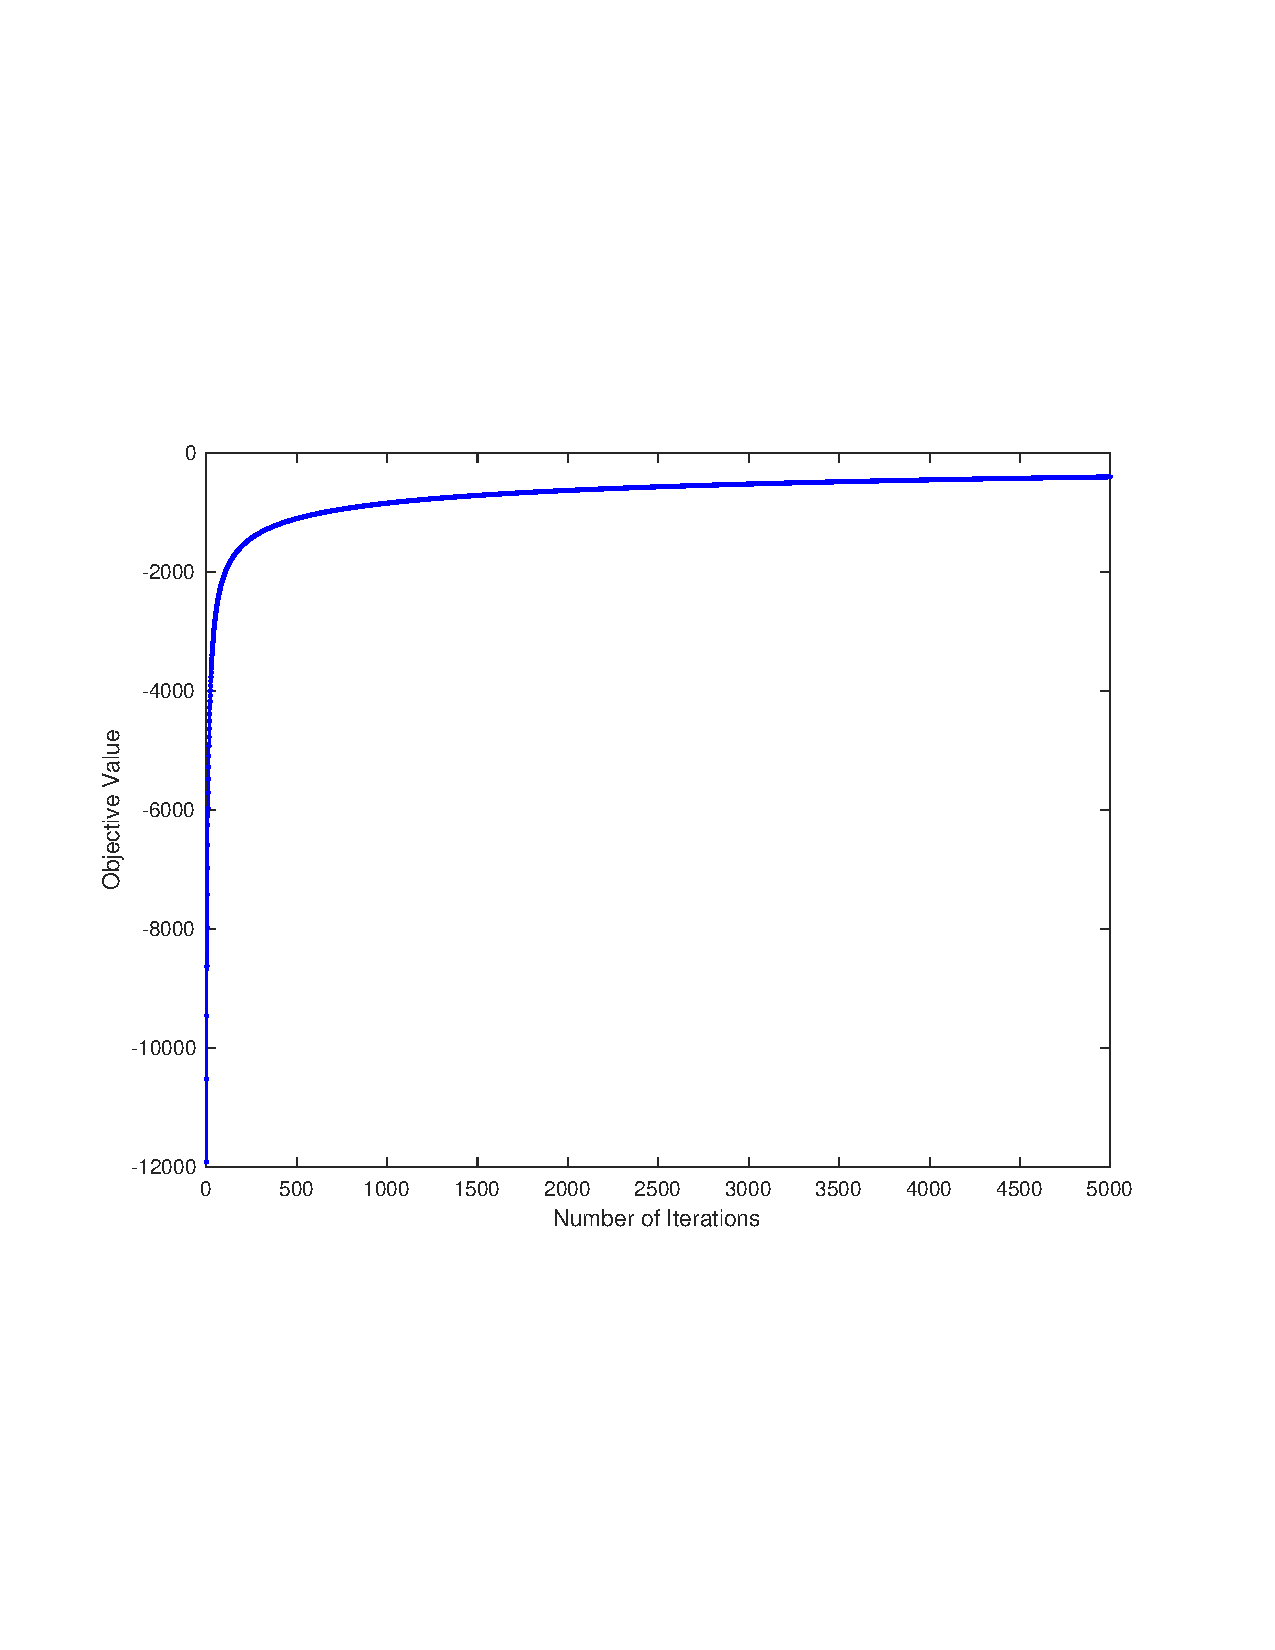
\includegraphics[width=.32\linewidth]{obj}
			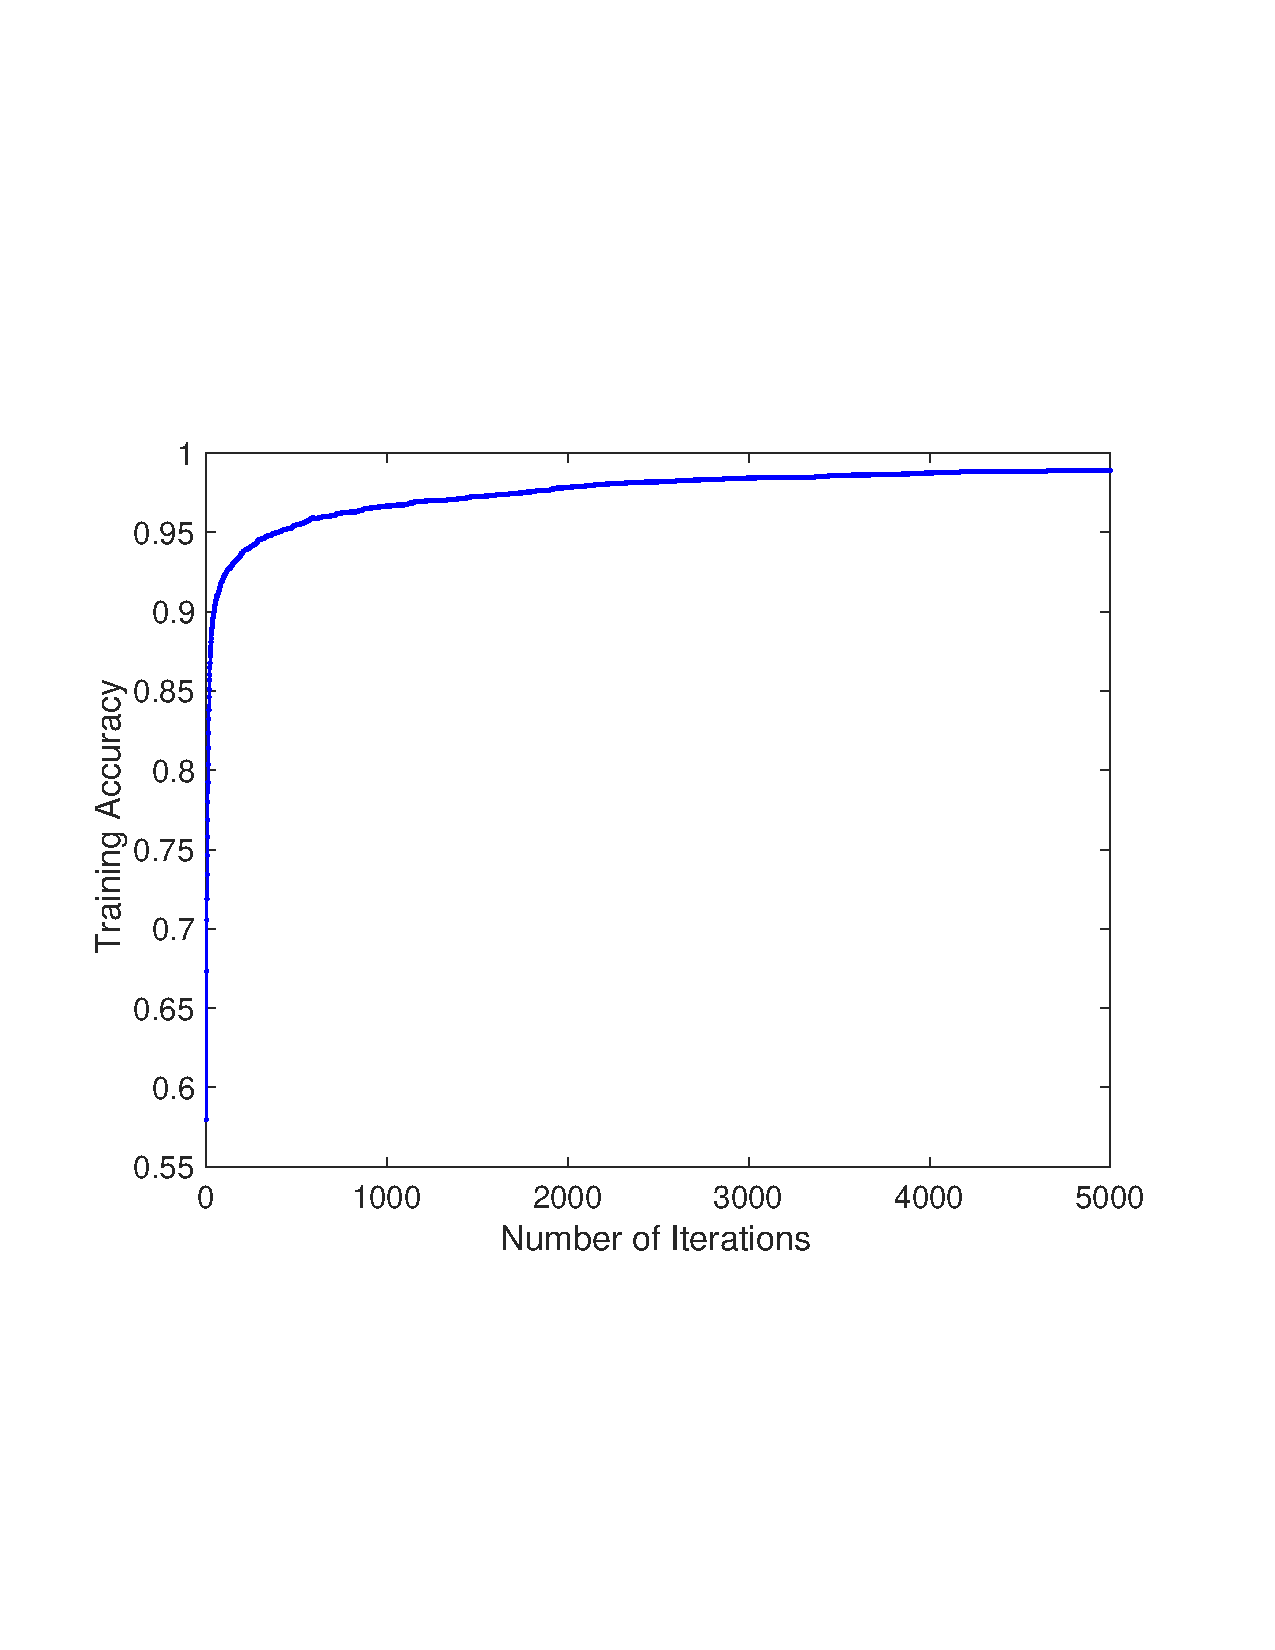
\includegraphics[width=.32\linewidth]{train_err}
			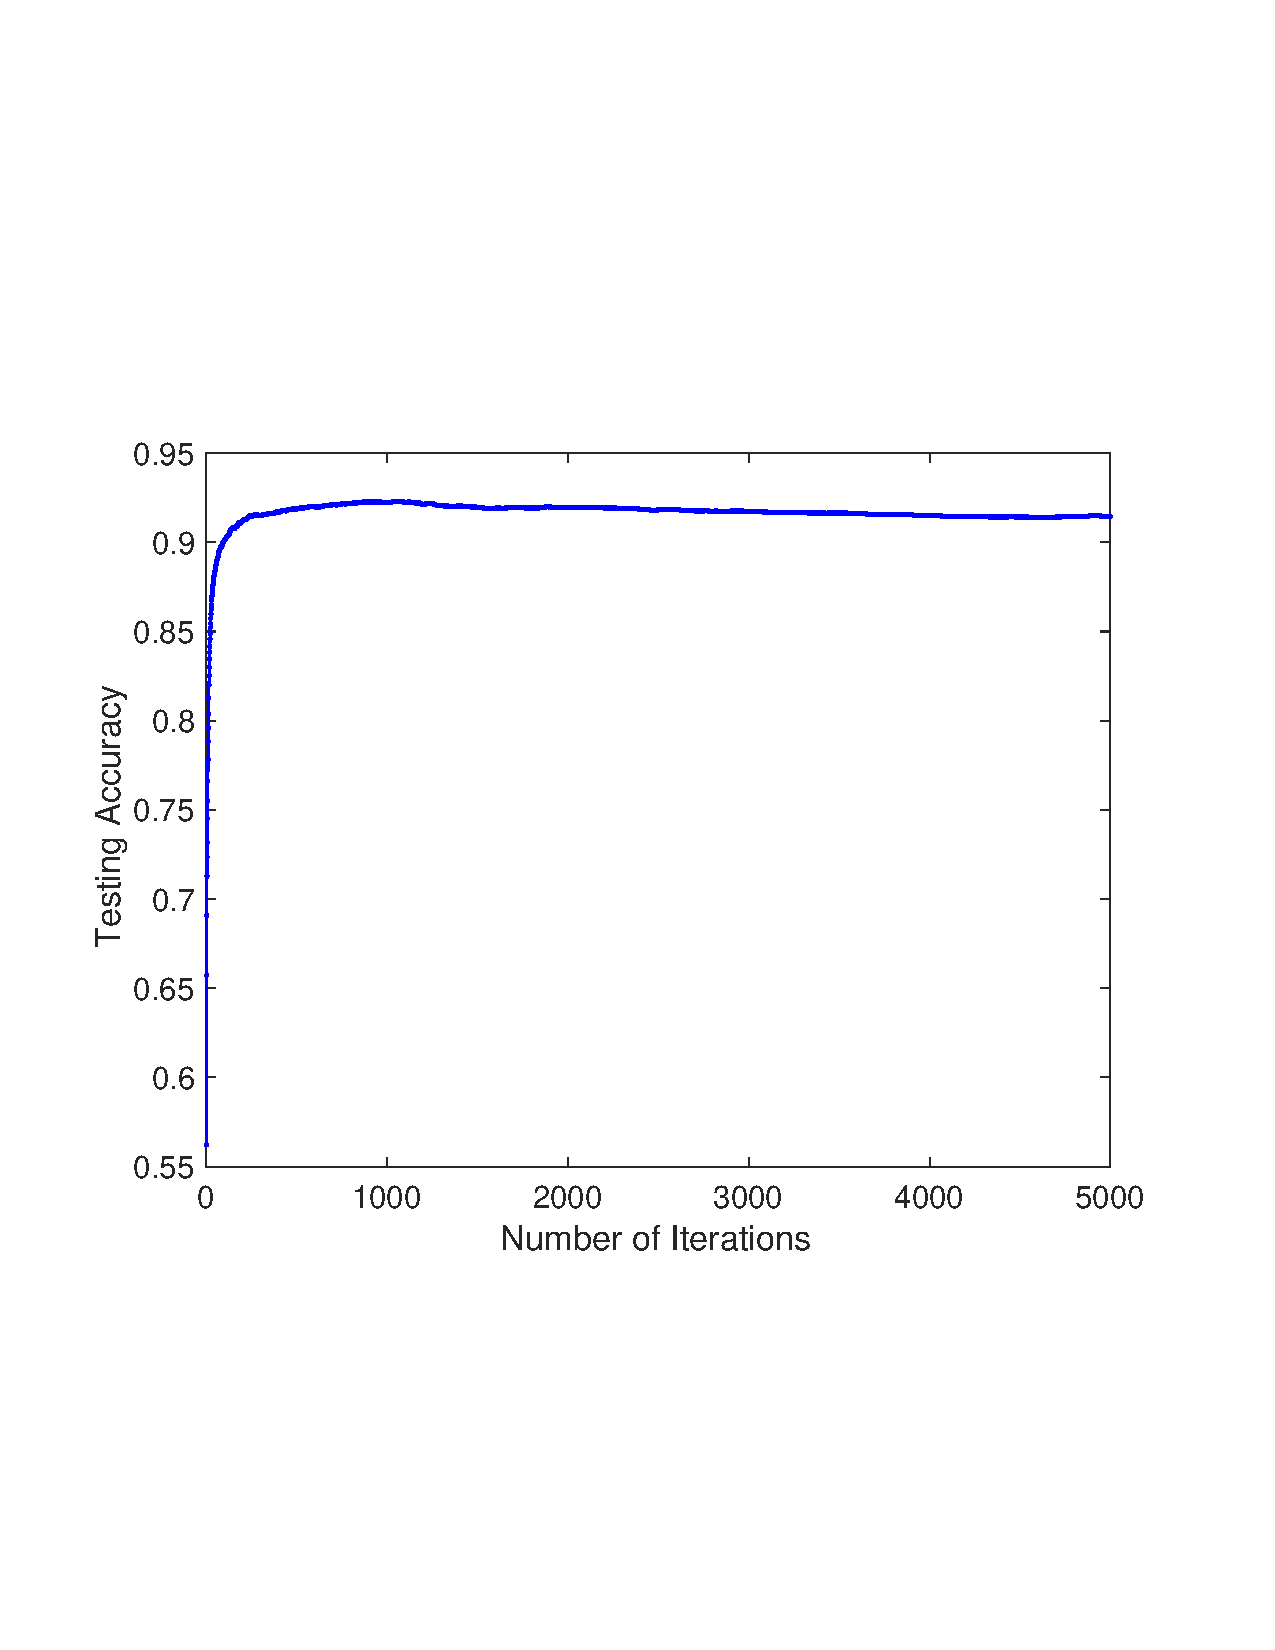
\includegraphics[width=.32\linewidth]{test_err}
		\end{figure}
		
		\item Now if we add the regularization term as Eq.(\ref{reg}), please show the final accuracy when $\lambda=\{0,1,10,100,200\}$ respectively.
		\begin{align*}
			\lambda = 0.1, acc = 0.914400\\
			\lambda = 1, acc = 0.915800\\
			\lambda = 10, acc = 0.919200\\
			\lambda = 100, acc = 0.897400\\
			\lambda = 200, acc = 0.881800\\
		\end{align*}
		\item What conclusion can we draw from the above experiments?
		penalty term can avoid overfitting on training data, but too large a penalty term will decrease the accuracy
	\end{enumerate}
\end{enumerate}

\end{document}
